\documentclass[a4paper,10pt]{article}
\usepackage[utf8]{inputenc}

\usepackage{graphicx}

\usepackage{amsmath}
\usepackage{amsfonts}
\usepackage{amssymb}

%opening
\title{Teoria para o cálculo da curva}
\author{Fernando Pujaico Rivera}

\begin{document}

\maketitle

\begin{abstract}

\end{abstract}


\section{Calculando o peço dos cúmulos}
\label{sec:cumulos}
Dada uma imagem  em branco e preto ($\mathbf{M}$), como mostrado na
Figura \ref{fig:moticacion}, 
\begin{figure}[!htb]
\centering
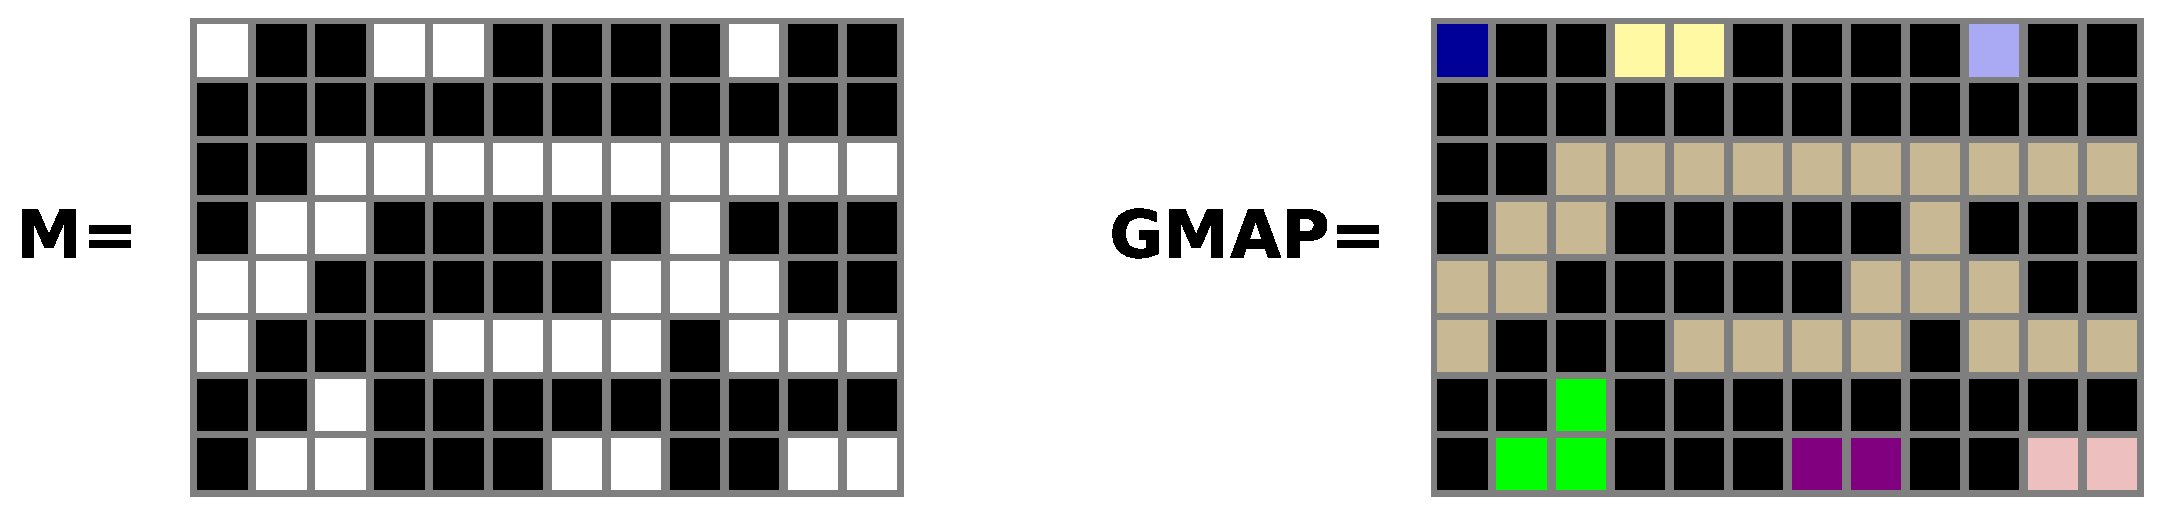
\includegraphics[scale=0.33]{moticacion.eps}
\caption{Imagem em branco e preto ($\mathbf{M}$), Imagem com cúmulos formados 
por grupos de pixels brancos ($\mathbf{GMAP}$) }
\label{fig:moticacion}
\end{figure}
com valores binários 
onde os pixels com cor branca tem valor $1$ e com cor preta $0$. 
Se desejamos obter uma imagem com cúmulos formados pelos grupos de pixels brancos ($\mathbf{GMAP}$); onde 
cada pixel é mapeado com um índice $ID$ ( na figura este $ID$ está representado 
com uma cor); devemos seguir o procedimento das seguintes seções.

\subsection{Modelando o problema}
\label{subsec:part1}

Nosso problema principal é obter, a partir de uma matriz $\mathbf{M}$, 
 uma matriz $\mathbf{GMAP}$ onde cade elemento contem
o índice do cúmulo ao qual pertence, como mostra a Figura \ref{fig:moticacion}.
Assim, pra cumprir este objetivo são usadas as funções $funA$ e $funB$, como mostra  a
Figura \ref{fig:modelocumulos}, onde são analisadas de maneira sequencial as colunas $\mathbf{M}(:,i)$ da
matriz $\mathbf{M}$, desde $i=0$ ate $i=N_{col}-1$, 
\begin{figure}[!htb]
\centering
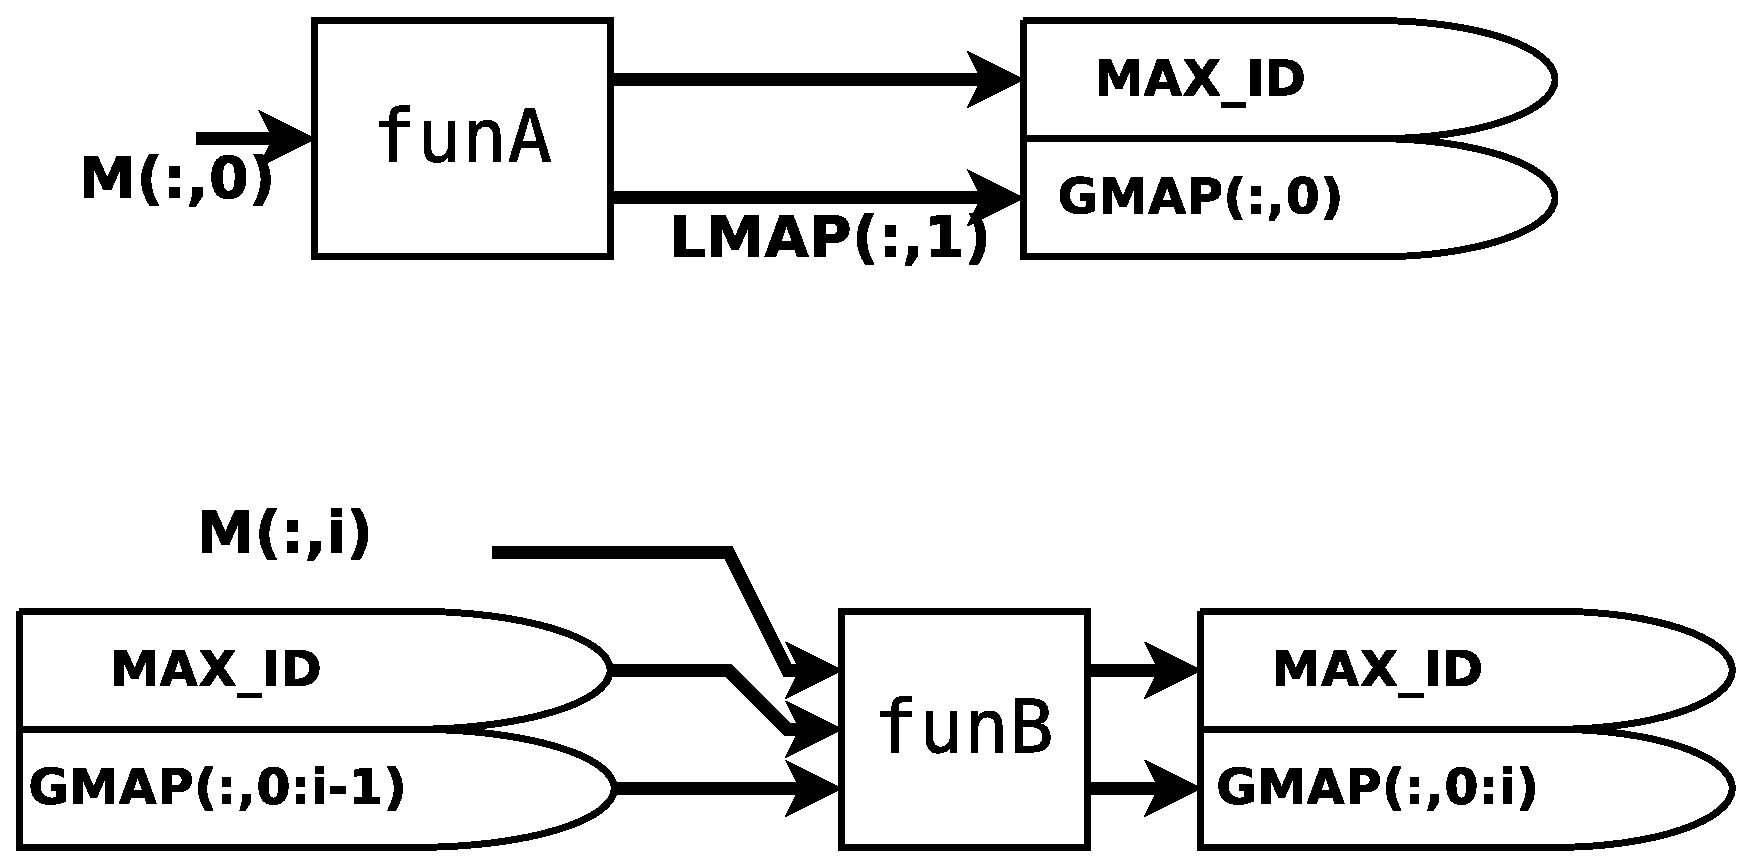
\includegraphics[scale=0.25]{DiagramaCompleto.eps}
\caption{Diagrama de fluxo del algoritmo de criação de cúmulos }
\label{fig:modelocumulos}
\end{figure}

A função $funA$ recebe como parâmetro de entrada a coluna $\mathbf{M}(:,0)$
(primeira coluna da matriz $\mathbf{M}$)
e retorna o valor dos índices em $\mathbf{GMAP}(:,0)$,
adicionalmente a função retorna o valor do maior índice atribuído nas operações ($MAX\_ID$).

Por outro lado a função $funB$ recebe como parâmetros de entrada a $i$-essima 
coluna ($\mathbf{M}(:,i)$) de $\mathbf{M}$, o mapa de índices $\mathbf{GMAP}(:,0:(i-1))$
que abrange informações de índice desde a primeira coluna ate a $(i-1)$-essima 
o valor do maior índice conhecido ate o momento, a função retorna
o a matriz $\mathbf{GMAP}(:,0:i)$ com os dados dos índices desde a primeira coluna ate a $i$-essima,
adicionalmente a função retorna o valor do maior índice atribuído nas operações ($MAX\_ID$).

\subsubsection{Algoritmo da função $funA$}
\label{subsubsec:funA}
A função $funA$ recebe um vetor coluna $\mathbf{V}$ com uns e zeros, como é exemplificado na
Figura \ref{fig:funA}, na saída a função retorna um vetor $\mathbf{LMAP}$ com o mesmo tamanho
porem com elementos com valores inteiros, representado estes o mapeamento dos índices dos elementos em $\mathbf{V}$,
\begin{figure}[!htb]
\centering
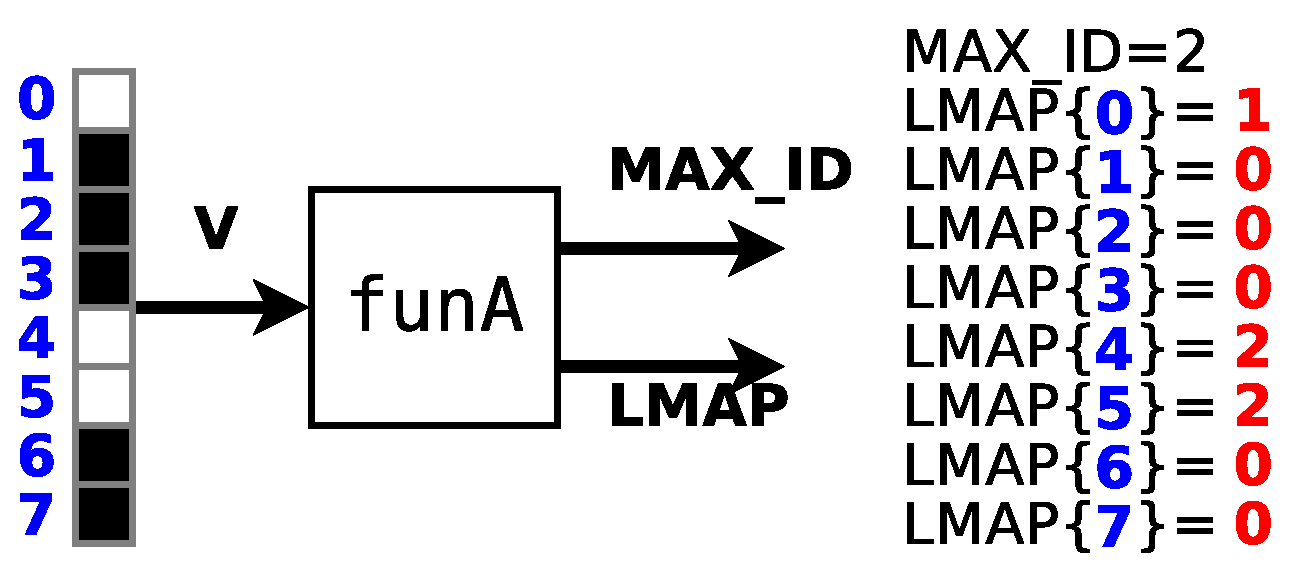
\includegraphics[scale=0.33]{funA.eps}
\caption{Descrição da função $funA$ }
\label{fig:funA}
\end{figure}
os elementos em $\mathbf{V}$ com valor zero recebem automaticamente um índice de valor $0$,
já se uma região de uns em $\mathbf{V}$, estão isolados, estes recebem em $\mathbf{LMAP}$ um índice
com um valor maior em uma unidade do ultimo índice achado; a função $funA$ também retorna
 o máximo índice estabelecido ($MAX\_ID$).

\subsubsection{Algoritmo da função $funB$}
\label{subsubsec:funB}
A função $funB$ recebe como parâmetros de entrada, um vetor $\mathbf{M}(:,i)$ correspondente a 
$i$-essima coluna da matriz $\mathbf{M}$, uma matriz $\mathbf{GMAP}(:,0:(i-1))$ com o mapa de grupos
desde a primeira coluna ate a $(i-1)$-essima coluna da matriz $\mathbf{GMAP}$, 
e o máximo índice $MAX\_ID$ nos elementos da matriz $\mathbf{GMAP}(:,0:(i-1))$, 
como é exemplificado na
Figura \ref{fig:funB}. Na saída a função retorna uma matriz $\mathbf{GMAP}(:,0:i)$ com o mapa de grupos
desde a primeira coluna ate a $i$-essima coluna da matriz $\mathbf{GMAP}$, 
e o novo máximo índice $MAX\_ID$ nos elementos da matriz $\mathbf{GMAP}(:,0:i)$.
\begin{figure}[!htb]
\centering
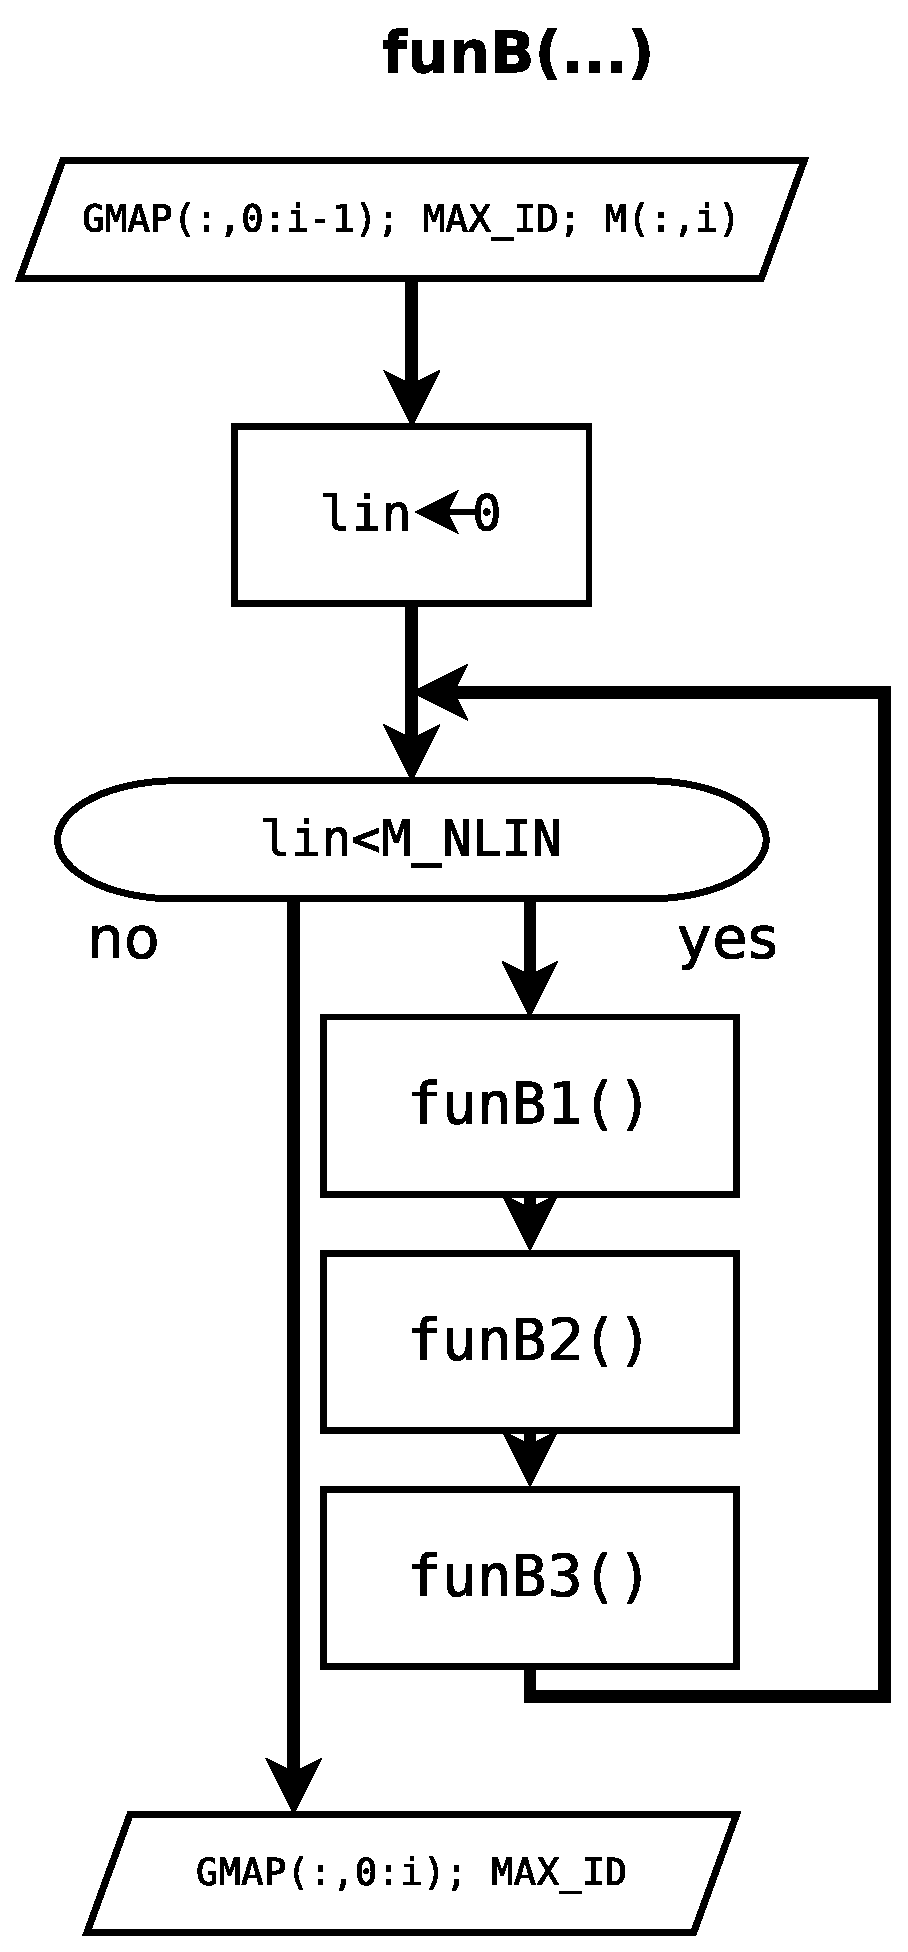
\includegraphics[scale=0.25]{funB.eps}
\caption{Descrição da função $funB$ }
\label{fig:funB}
\end{figure}
A função $funB$ analisa os elementos do vetor $\mathbf{M}(:,i)$, desde a primeira
linha ate a linha $M\_NLIN$, mediante as funções auxiliares $funB1$, $funB2$ e $funB3$,
estas funções modificam o conteúdo da matriz $\mathbf{GMAP}(:,0:i)$ e a variável $MAX\_ID$.

\textbf{Algoritmo da função $funB1$}:
A função recebe como para metros de entrada os vetores $\mathbf{M}(:,i)$, $\mathbf{GMAP}(:,i)$
e uma variável com a linha $lin$ onde inciara o analises.
Se existem zeros em $\mathbf{M}(:,i)$, então se escrevem zeros nos elementos na mesma posição 
do vetor $\mathbf{GMAP}(:,i)$.
Figura \ref{fig:funB1}
\begin{figure}[!htb]
\centering
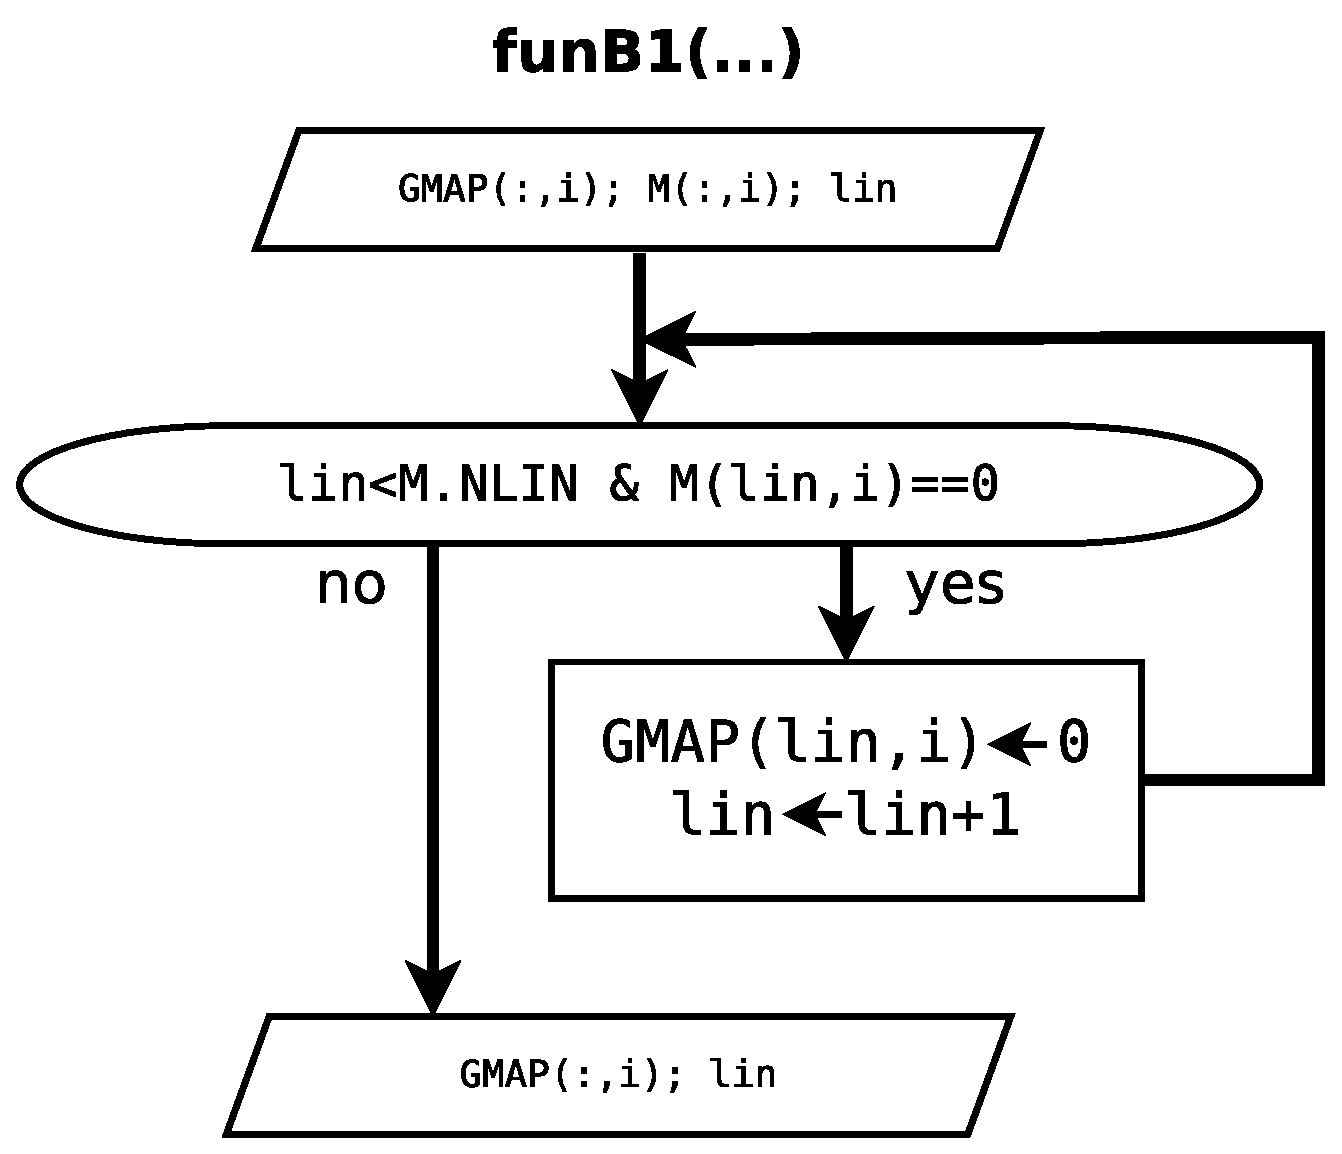
\includegraphics[scale=0.25]{funB1.eps}
\caption{Descrição da função $funB1$ }
\label{fig:funB1}
\end{figure}

\textbf{Algoritmo da função $funB2$}:
Verifico si existem uns; e acho o conjunto de ID globais ligados a esse grupo de uns,
adicionalmente é contada a quantidade de uns.
Figura \ref{fig:funB2}
\begin{figure}[!htb]
\centering
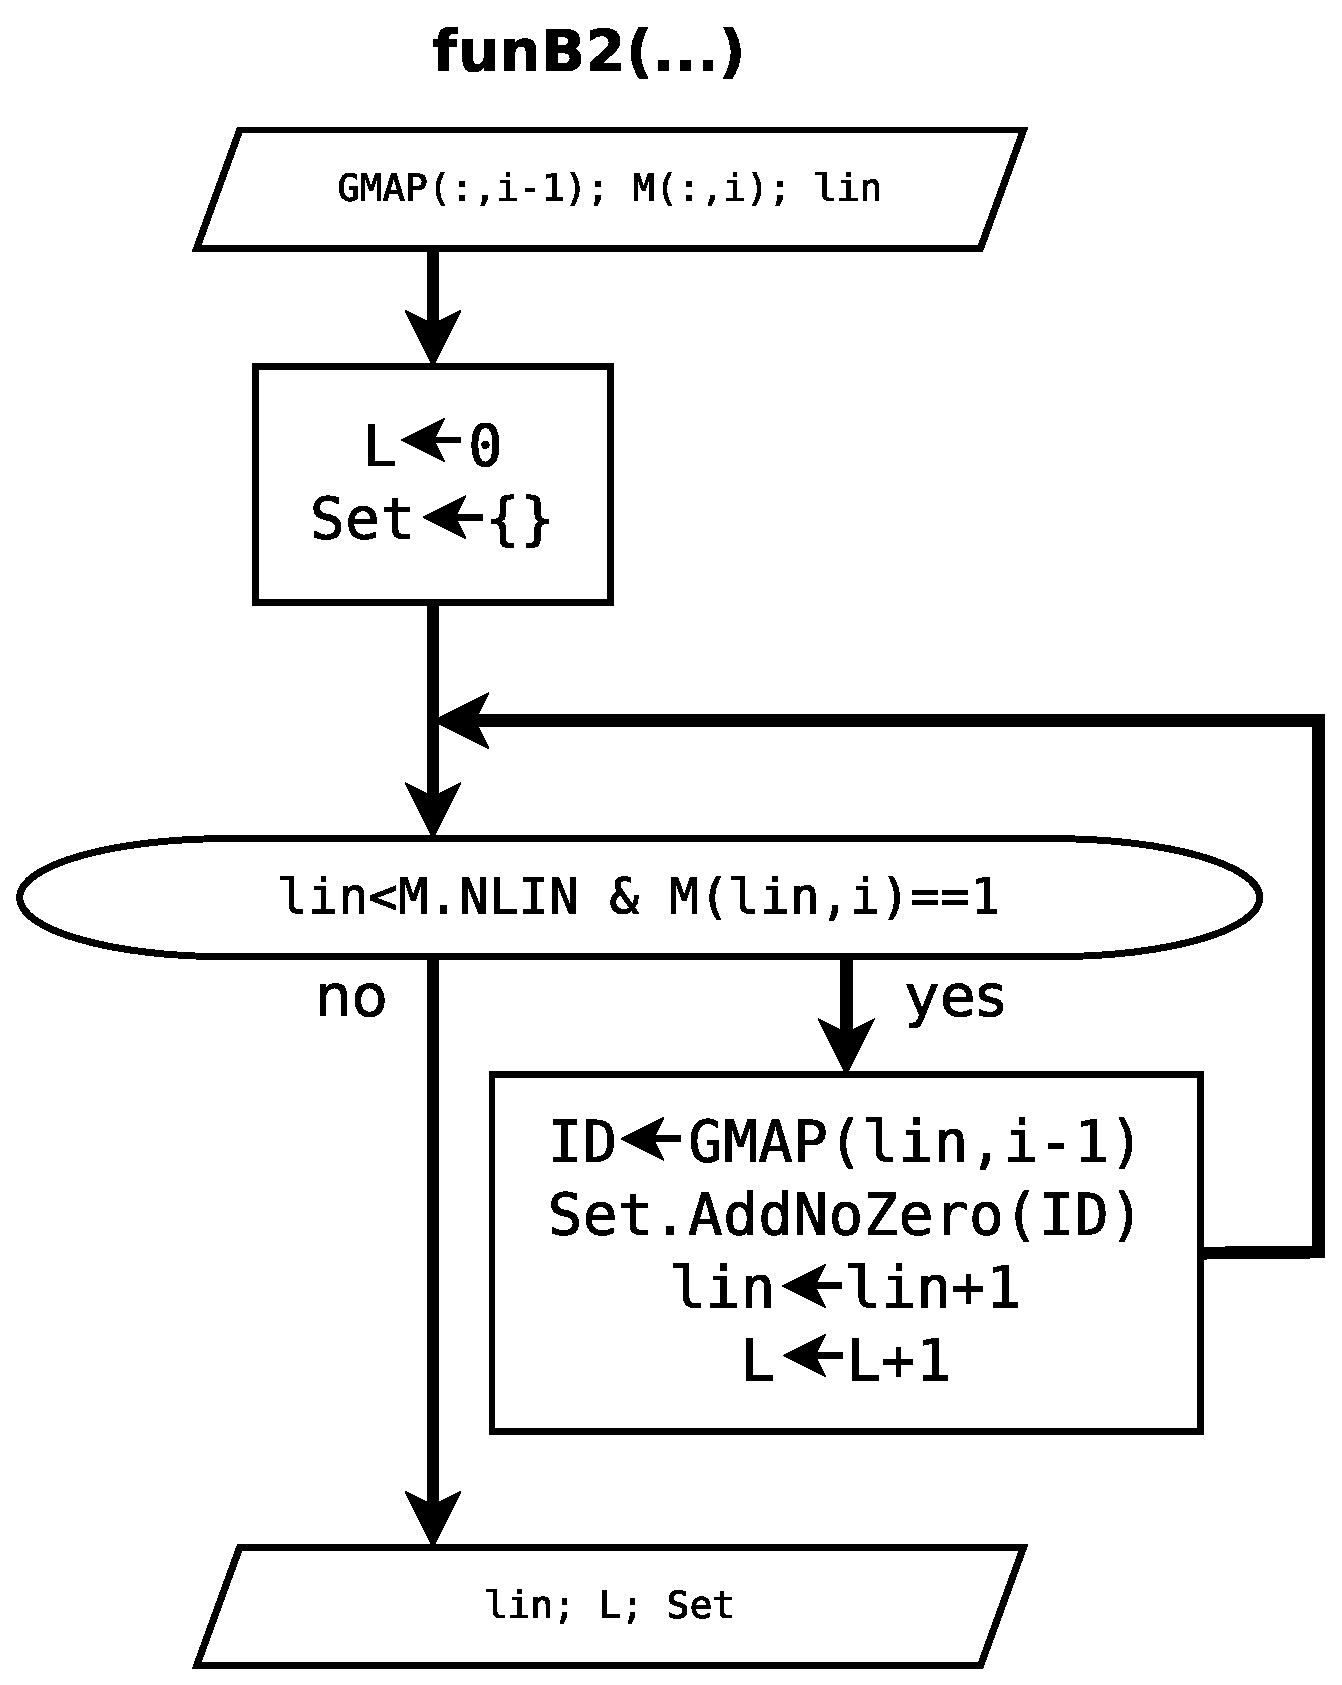
\includegraphics[scale=0.25]{funB2.eps}
\caption{Descrição da função $funB$ }
\label{fig:funB2}
\end{figure}

\subsection{Calculando a matriz $\mathbf{GMAP}$ e $\mathbf{W}$}

\section{least-squares fitting of cubic splines (Method 1)}
\label{sec:spline3method1}

Este trabalho mostra como calcular o encaixe de uma curva $y=f(x)$ 
mediante mínimos quadrados sobre um conjunto de $N$ pontos $(x_n,y_n)$; 
$\forall n \in \mathtt{Z},~0\leq n < N$; tendo
cada ponto uma importância de $w_n$.
Onde a curva 
$y=f(x)$ esta composta de um grupo de $M$ splines cúbicos, 
como o exemplo da Figura \ref{fig:leastmeanspline3}.
\begin{figure}[!htb]
\centering
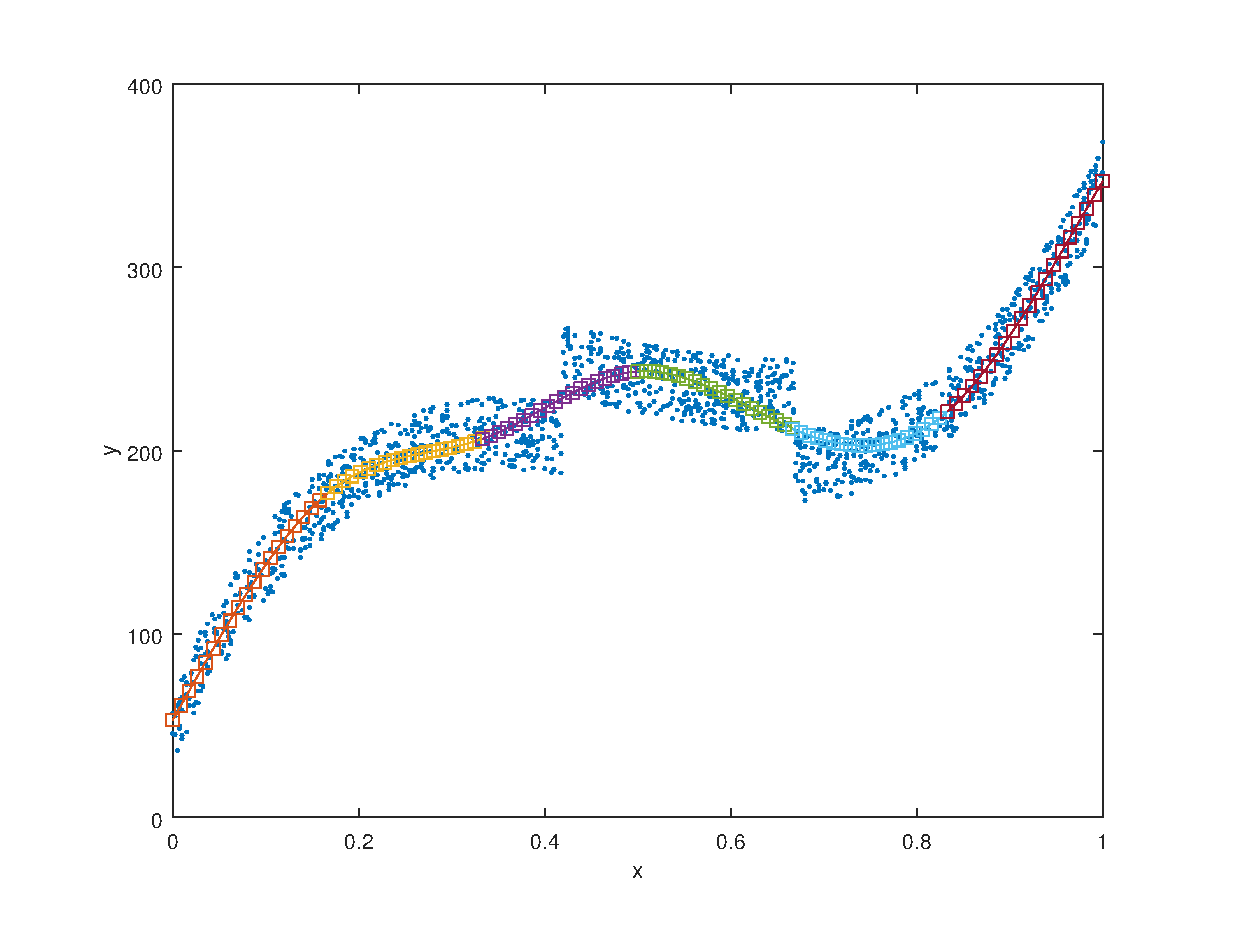
\includegraphics[scale=0.33]{splines3demo.eps}
\caption{Fitting of $M=6$ cubic splines in a set of $N=500$ pontos $(x_n,y_n)$.}
\label{fig:leastmeanspline3}
\end{figure}

Os splines tem seus limites de domínio, nas posições onde $x$ tem valores 
$\varepsilon_{0}, \varepsilon_{1}, \varepsilon_{2}, ..., \varepsilon_{M}$. 


Assim, usando as variáveis 
$\mathbf{E}=\left(\begin{matrix}\varepsilon_0 & \varepsilon_1 & ...  & \varepsilon_{M}\end{matrix}\right)^T$ e
$\mathbf{P}=\left(\begin{matrix}P_0 & P_1 & ...  & P_{4M-1}\end{matrix}\right)^T$,
podemos definir as seguintes funções,
\begin{equation}
 G(x,a,b)= \left\{\begin{matrix}
1 & if &  a \leq x \leq b \\ 
0 & if & other~case
\end{matrix}\right.
\end{equation}
\begin{equation}
 S_k(x,\mathbf{P})=P_{4k}~x^3+P_{1+4k}~x^2+P_{2+4k}~x+P_{3+4k},
\end{equation}
de modo que
\begin{equation}
 f(x,\mathbf{P},\mathbf{E})=\sum_{k=0}^{M-1} S_k(x,\mathbf{P})G(x,\varepsilon_{k},\varepsilon_{k+1})  
\end{equation}

\subsection{Modelando o problema}
\label{subsec:all}
Para poder calcular o vetor $\mathbf{P}=\left(\begin{matrix}P_0 & P_1 & P_2 & ...  & P_{4M-1}\end{matrix}\right)^T$, 
do problema spline descrito  na Seção \ref{sec:spline3method1}, a partir dos dados $(x_n,y_n,w_n)$; 
$\forall n \in \mathtt{Z},~0\leq n < N$ e escolhidos os valores $\mathbf{E}=\left(\begin{matrix}\varepsilon_0 & \varepsilon_1 & ...  & \varepsilon_{M}\end{matrix}\right)^T$;
ordenamos nossos dados nos seguintes vetores coluna:
\begin{equation}
\mathbf{X}=\left(\begin{matrix}\mathbf{X}_0 \\ \mathbf{X}_1 \\ \vdots  \\ \mathbf{X}_{M-1}\end{matrix}\right),~~
\mathbf{Y}=\left(\begin{matrix}\mathbf{Y}_0 \\ \mathbf{Y}_1 \\ \vdots  \\ \mathbf{Y}_{M-1}\end{matrix}\right),~~
\mathbf{W}=\left(\begin{matrix}\mathbf{W}_0 \\ \mathbf{W}_1 \\ \vdots  \\ \mathbf{W}_{M-1}\end{matrix}\right),
\end{equation}
onde os elementos de $\mathbf{X}_m$,$\mathbf{Y}_m$,$\mathbf{W}_m$ representam os valores de $(x_n,y_n,w_n)$
que cumprem $\varepsilon_m \leq x_n \leq \varepsilon_{m+1}$.


\subsubsection{Equação que relacionam os dados }
\label{subsubsec:partz}
Os dados $(x_n,y_n)$ são agrupados em $\mathbf{Y}=\mathbf{A}\mathbf{P}$, onde,
\begin{equation}
\mathbf{A}_m =\left(\begin{matrix}
\mathbf{X}_m^3 & \mathbf{X}_m^2 & \mathbf{X}_m & \mathbf{1}
\end{matrix}\right)
\end{equation}
\begin{equation}
\mathbf{A} =\left(\begin{matrix}
\mathbf{A}_0 & \mathbf{0}   & \mathbf{0}   & \dots & \mathbf{0} \\
\mathbf{0}   & \mathbf{A}_1 & \mathbf{0}   & \dots & \mathbf{0} \\
\mathbf{0}   & \mathbf{0}   & \mathbf{A}_2 & \dots & \mathbf{0} \\
\mathbf{0}   & \mathbf{0}   & \mathbf{0}   & \dots & \mathbf{A}_{M-1} \\
\end{matrix}\right)
\end{equation}

\subsubsection{Equação de continuidade dos splines consecutivos}
\label{subsubsec:part0}
Dados os polinômios $S_{k-1}(x,\mathbf{P})$ e $S_{k}(x,\mathbf{P})$ do $(k-1)$-essimo e $k$-essimo spline,
respetivamente. Podemos igualar ambos polinômios para garantir a continuidade dos splines em $x=\varepsilon_{k}$, 
de modo que,
\begin{equation}
 S_{k-1}(\varepsilon_{k},\mathbf{P})=S_{k}(\varepsilon_{k},\mathbf{P})
\end{equation}
Assim, agrupando as equações dos polinômios de  $0<k<M$, obtemos $\mathbf{0}=\mathbf{B}_0 \mathbf{P}$, onde,
\begin{equation}
\mathbf{B}_0 =\left(\begin{matrix}
\mathbf{E}_1 & -\mathbf{E}_1   & \mathbf{0}    &  \mathbf{0}   & \dots & \mathbf{0} & \mathbf{0}\\
\mathbf{0}   &  \mathbf{E}_2   & -\mathbf{E}_2 &  \mathbf{0}   & \dots & \mathbf{0} & \mathbf{0}\\
\mathbf{0}   &  \mathbf{0}     &  \mathbf{E}_3 & -\mathbf{E}_3 & \dots & \mathbf{0} & \mathbf{0}\\
\vdots       &  \vdots         &  \vdots       &  \vdots       & \dots & \vdots     & \vdots\\
\mathbf{0}   &  \mathbf{0}     &  \mathbf{0}   &  \mathbf{0}   & \dots & \mathbf{E}_{M-1} & -\mathbf{E}_{M-1} \\
\end{matrix}\right),
\end{equation}
usando como variável auxiliar,
\begin{equation}
\mathbf{E}_k =\left(\begin{matrix}
\varepsilon^3_k & \varepsilon^2_k   & \varepsilon_k & 1  \\
\end{matrix}\right).
\end{equation}

\subsubsection{Equação de continuidade da 1ra derivada dos splines consecutivos}
\label{subsubsec:part1}
Dados os polinômios $S_{k-1}(x,\mathbf{P})$ e $S_{k}(x,\mathbf{P})$ do $(k-1)$-essimo e $k$-essimo spline,
respetivamente. Podemos igualar a primeira derivada de  ambos polinômios para garantir a continuidade dos splines em $x=\varepsilon_{k}$, 
de modo que,
\begin{equation}
 \left.\frac{\partial~S_{k-1}(x,\mathbf{P})}{\partial x}\right|_{x=\varepsilon_{k}} = 
 \left.\frac{\partial~S_{k}  (x,\mathbf{P})}{\partial x}\right|_{x=\varepsilon_{k}}
\end{equation}
Assim, agrupando as equações dos polinômios de  $0<k<M$, obtemos $\mathbf{0}=\mathbf{B}_1 \mathbf{P}$, onde,
\begin{equation}
\mathbf{B}_1 =\left(\begin{matrix}
\partial\mathbf{E}_1 & -\partial\mathbf{E}_1   & \mathbf{0}    &  \mathbf{0}   & \dots & \mathbf{0} & \mathbf{0}\\
\mathbf{0}   &  \partial\mathbf{E}_2   & -\partial\mathbf{E}_2 &  \mathbf{0}   & \dots & \mathbf{0} & \mathbf{0}\\
\mathbf{0}   &  \mathbf{0}     &  \partial\mathbf{E}_3 & -\partial\mathbf{E}_3 & \dots & \mathbf{0} & \mathbf{0}\\
\vdots       &  \vdots         &  \vdots       &  \vdots       & \dots & \vdots     & \vdots\\
\mathbf{0}   &  \mathbf{0}     &  \mathbf{0}   &  \mathbf{0}   & \dots & \partial\mathbf{E}_{M-1} & -\partial\mathbf{E}_{M-1} \\
\end{matrix}\right),
\end{equation}
usando como variável auxiliar,
\begin{equation}
\partial\mathbf{E}_k =\left(\begin{matrix}
3\varepsilon^2_k & 2\varepsilon_k   & 1 & 0  \\
\end{matrix}\right).
\end{equation}

\subsubsection{Equação de continuidade da 2da derivada dos splines consecutivos}
\label{subsubsec:part2}
Dados os polinômios $S_{k-1}(x,\mathbf{P})$ e $S_{k}(x,\mathbf{P})$ do $(k-1)$-essimo e $k$-essimo spline,
respetivamente. Podemos igualar a segunda derivada de ambos polinômios para garantir a continuidade dos splines em $x=\varepsilon_{k}$, 
de modo que,
\begin{equation}
 \left.\frac{\partial^2~S_{k-1}(x,\mathbf{P})}{\partial x^2}\right|_{x=\varepsilon_{k}} = 
 \left.\frac{\partial^2~S_{k}  (x,\mathbf{P})}{\partial x^2}\right|_{x=\varepsilon_{k}}
\end{equation}
Assim, agrupando as equações dos polinômios de  $0<k<M$, obtemos $\mathbf{0}=\mathbf{B}_2 \mathbf{P}$, onde,
\begin{equation}
\mathbf{B}_2 =\left(\begin{matrix}
\partial^2\mathbf{E}_1 & -\partial^2\mathbf{E}_1   & \mathbf{0}    &  \mathbf{0}   & \dots & \mathbf{0} & \mathbf{0}\\
\mathbf{0}   &  \partial^2\mathbf{E}_2   & -\partial^2\mathbf{E}_2 &  \mathbf{0}   & \dots & \mathbf{0} & \mathbf{0}\\
\mathbf{0}   &  \mathbf{0}     &  \partial^2\mathbf{E}_3 & -\partial^2\mathbf{E}_3 & \dots & \mathbf{0} & \mathbf{0}\\
\vdots       &  \vdots         &  \vdots       &  \vdots       & \dots & \vdots     & \vdots\\
\mathbf{0}   &  \mathbf{0}     &  \mathbf{0}   &  \mathbf{0}   & \dots & \partial^2\mathbf{E}_{M-1} & -\partial^2\mathbf{E}_{M-1} \\
\end{matrix}\right),
\end{equation}
usando como variável auxiliar,
\begin{equation}
\partial^2\mathbf{E}_k =\left(\begin{matrix}
6\varepsilon_k & 2   & 0 & 0  \\
\end{matrix}\right).
\end{equation}


\subsection{Calculando os parâmetros $P_j$}
Agrupando os resultados da  Seção \ref{subsec:all}, 
podemos definir a seguinte equação,
\begin{equation}
\left(\begin{matrix}
\mathbf{Y} \\
\mathbf{0} \\
\mathbf{0} \\
\mathbf{0} 
\end{matrix}\right)
=\left(\begin{matrix}
\mathbf{A} \\
\mathbf{B}_0 \\
\mathbf{B}_1 \\
\mathbf{B}_2 
\end{matrix}\right) \mathbf{P}
\end{equation}
ou seu equivalente, $\mathbf{Z} = \mathbf{Q}  \mathbf{P}$. Onde a única incógnita é $\mathbf{P}$.

Para resolver este problema aplicamos $LMS$ (Least Mean Square) a equação, para isso
definimos a  regra de minimização $e(\mathbf{P})$,
\begin{equation}
 e(\mathbf{P})=||\mathbf{Z} -\mathbf{Q}  \mathbf{P} ||_{diag(\mathbf{W})}^2+\alpha || \mathbf{P}-\mathbf{P}_{*} ||.
\end{equation}
Onde $\mathbf{P}_{*}$ é o valor de $\mathbf{P}$ na iteração anterior. Assim, aplicando
$LMS$ e a regularização de Tikhonov, o mínimo valor de $\mathbf{P}$ se obtêm iterativamente usando a seguinte equação
\begin{equation}
\mathbf{P}_{k+1}= \mathbf{P}_{k}+ \left[ \mathbf{Q}^T diag(\mathbf{W})\mathbf{Q} +\alpha \mathbf{I} \right]^{-1} \mathbf{Q}^T diag(\mathbf{W})  \left[ \mathbf{Z}-\mathbf{Q}  \mathbf{P}_{k} \right]
\end{equation}
ate que os vetores $\mathbf{P}_{k}$ e $\mathbf{P}_{k+1}$ sejam muito próximos.

\end{document}
